% !TeX root = Protokoll.tex
Der größte Anteil aller Festkörper, besitzt einen kristallinen Aufbau. Dies bedeutet die Atome sind räumlich periodisch angeordnet. Um die Kristalleigenschaften zu diskutieren wird ein einzelner Kristall oder auch Einkristall betrachtet, weil sich die anisotropen Eigenschaften in Kristallen die sich im polykristallinem Zustand befinden heraus Mitteln. Um Kristalle Vermessen zu können, werden Strahlen benötigt deren Wellenlänge sich in der Größenordnung des Atomabstands befinden. Bei der Dybe-Scherrer-Methode werden dafür Röntgenstrahlen verwendet.
\subsection{Kristallstrukturen}
\begin{figure}[h!]
	\centering
	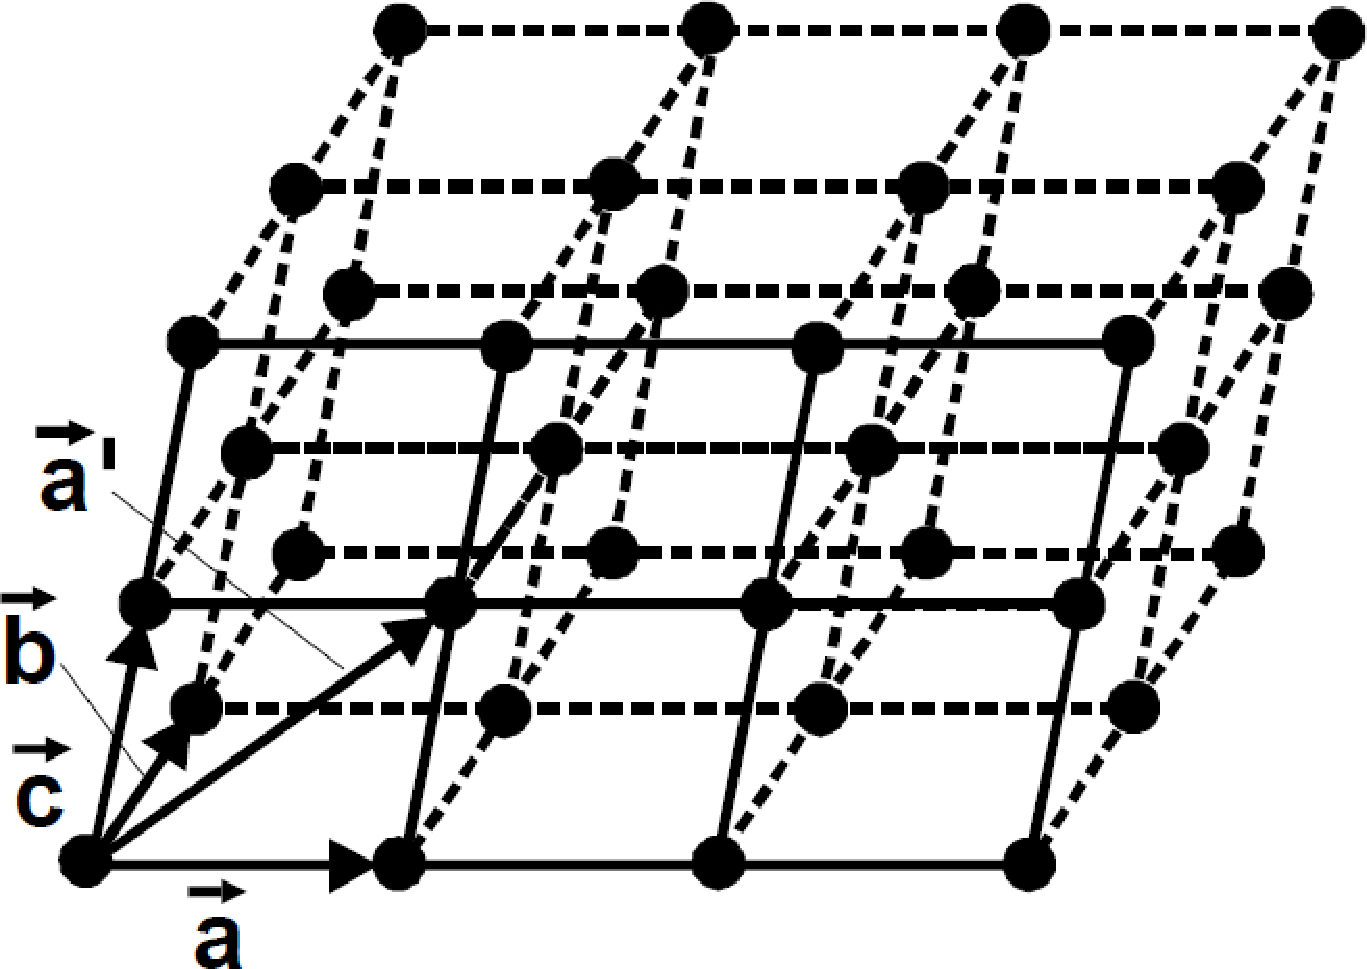
\includegraphics[scale = 0.4]{../Grafiken/Gitter.pdf}
	\caption{Eine Veranschaulichung für ein Kristallgitter.\cite{V41}}
	\label{fig:BeispielGitter}
\end{figure}
Ein Kristall kann als dreidimensionales Gitter beschrieben werden. Die Eckpunkte sind die Basis und beschreiben die Positionen der Atome oder von Atomgruppen.
Aufgrund der Periodizität des Kristalls, lässt er sich vollständig durch drei Vektoren $\vec{a}$, $\vec{b}$ und $\vec{c}\ $ beschreiben. Wie schon in \ref{fig:BeispielGitter} zu sehen ist die Wahl der Vektoren nicht eindeutig. Alle Gitterpunkte werden durch den Vektor 
\begin{align}
	\vec{t}= n_1\cdot \vec{a}+n_2\cdot\vec{b}+n_3\cdot\vec{c}
\end{align}
erreicht, dabei ist $n_i$ ganzzahlig. Das Gitter kann um den Vektor $\vec{t}$ verschoben werden und das Gitter wird in sich selbst überführt, dies wird als Translationssymmetrie bezeichnet. Die Elementarzelle ist die kleinste Einheit, die die Kristallstruktur beinhaltet. Sind in der Elementarzelle nur die Atome auf den acht Eckpunkten, dann liegt eine primitive Elementarzelle vor.\\
Nach den bisherigen Annahmen für einen Kristall gibt es unendlich viele verschiedene, weil es keine Bedingung für die Länge der Vektoren gibt und den Winkeln zwischen ihnen. Durch Betrachtung von Symmetrien können dir Anzahl an Gitter Eingeschränkt werden. Dazu wird Spiegelung, Inversion oder Rotationen betrachtet. Dadurch bleiben nur noch die 14 Bravis-Gitter übrig, die sich in 7 Gittersysteme einteilen lassen, aufgrund der verschiedenen Elementarzellen.
In diesem Versuch wird eine Auswahl betrachtet.\\
\begin{table}[h!]
	\centering
	\begin{tabular}{c|c|c}
		System 	& Bezeichnung 				& Eigenschaften\\\hline
				& kubisch-primitiv			& $a=b=c$\\
		kubisch & kubisch-flächenzentriert	& $\alpha=\beta=\gamma=90^\circ$\\
				& kubisch-raumzentriert		&\\\hline
		hexagonal& hexagonal-primitiv		&$a=b=c$\\
				&							&$\alpha = \beta =90^\circ$, $ \gamma=120^\circ$
	\end{tabular}
	\caption{Dies ist eine Kurze Übersicht für die Kristalltypen die in diesem Versuch betrachtet werden\cite{V41}.}
	\label{tab:Kristalltypen}
\end{table}\\
Als erstes wird der kubisch-primitive Kristall (sc) betrachtet. Dieser Kristall ist die primitive Elementarzelle, das heißt nur die acht Atome auf den Ecken gehören dazu. Um auf die Anzahl an Atomen innerhalb der Elementarzelle zu kommen werden die Atome als harte Kugeln betrachtet und der Volumenanteil der Kugel die innerhalb der Elementarzelle sind werden aufsummiert. Für das sc-Gitter bedeutet das 1 und der Abstand der nächsten Atom ist $a$.\\
Als zweites wird der kubisch-raumzentrierte Kristall betrachtet. Die Anzahl der Atome in Gitter sind zwei, die acht Eckpunkte zu je einem achtel und eines in der Mitte des Würfels. Der Abstand zum nächsten Nachtberns beträgt $\sqrt{3}a/2$. Die Positionen der Basis-Atome kann somit geschrieben werden als
\begin{align}
	\left (0 , 0 , 0 \right)\ \text{und}\ \left(\frac{1}{2},\frac{1}{2},\frac{1}{2}\right).
\end{align}
Als letztes der kubischen Kristallen wird die kubisch-flächenzentrierte (fcc) Struktur betrachtet.
Neben den Eckpunkten gibt es noch sechs weitere Atome die sich mittig auf den Flächen des Würfels befinden. Daraus resultiert das in der Zelle vier Atome sind. Der Abstand der nächsten Nachtberns ist somit $\sqrt{2}a/2$.
Die Basis kann geschrieben werden als
\begin{align}
	\left( 0, 0, 0\right),\ \left( \frac{1}{2},\frac{1}{2},0\right),\ \left(\frac{1}{2}, 0 , \frac{1}{2}\right)\ \text{und}\ \left(0,\frac{1}{2},\frac{1}{2}\right).
\end{align}






\subsection{Netzebenen}
